\documentclass[a4paper, 10pt, twoside]{article}

\usepackage[top=1in, bottom=1in, left=1in, right=1in]{geometry}
\usepackage[utf8]{inputenc}
\usepackage[spanish, es-ucroman, es-noquoting]{babel}
\usepackage{setspace}
\usepackage{fancyhdr}
\usepackage{lastpage}
\usepackage{amsmath}
\usepackage{amsfonts}
\usepackage{amsthm}
\usepackage{verbatim}
\usepackage{fancyvrb}
\usepackage{graphicx}
\usepackage{float}
\usepackage{enumitem} % Provee macro \setlist
\usepackage{tabularx}
\usepackage{multirow}
\usepackage{hyperref}
\usepackage{lscape}
\usepackage{xspace}
\usepackage{qtree}
\usepackage[toc, page]{appendix}


%%%%%%%%%% Constantes - Inicio %%%%%%%%%%
\newcommand{\titulo}{Trabajo Práctico 2}
\newcommand{\materia}{ISW II}
\newcommand{\integrantes}{Almansi · Gasperi · `El capo del sorting` Russo · Tagliavini}
\newcommand{\cuatrimestre}{Primer Cuatrimestre de 2015}
%%%%%%%%%% Constantes - Fin %%%%%%%%%%


%%%%%%%%%% Configuración de Fancyhdr - Inicio %%%%%%%%%%
\pagestyle{fancy}
\thispagestyle{fancy}
\lhead{\titulo\ · \materia}
\rhead{\integrantes}
\renewcommand{\footrulewidth}{0.4pt}
\cfoot{\thepage /\pageref{LastPage}}

\fancypagestyle{caratula} {
   \fancyhf{}
   \cfoot{\thepage /\pageref{LastPage}}
   \renewcommand{\headrulewidth}{0pt}
   \renewcommand{\footrulewidth}{0pt}
}
%%%%%%%%%% Configuración de Fancyhdr - Fin %%%%%%%%%%


%%%%%%%%%% Miscelánea - Inicio %%%%%%%%%%
% Evita que el documento se estire verticalmente para ocupar el espacio vacío
% en cada página.
\raggedbottom

% Separación entre párrafos.
\setlength{\parskip}{0.5em}

% Separación entre elementos de listas.
\setlist{itemsep=0.5em}

% Asigna la traducción de la palabra 'Appendices'.
\renewcommand{\appendixtocname}{Apéndices}
\renewcommand{\appendixpagename}{Apéndices}

\newcommand{\diagrama}[1]{
  \begin{center}
    \includegraphics[width=16cm]{#1}
  \end{center}
}

\newcommand{\diagramadeancho}[2]{
  \begin{center}
    \includegraphics[width=#1]{#2}
  \end{center}
}

\newcommand{\riesgo}[7]{
  \underline{Riesgo {#1}:}
  \begin{itemize}   
    \item \textbf{Descripción:} {#2}
    \item \textbf{Probablidad:} {#3}
    \item \textbf{Impacto:} {#4}
    \item \textbf{Exposición:} {#5}
    \item \textbf{Mitigación:} {#6}
    \item \textbf{Plan de contingencia:} {#7}
  \end{itemize}
}

\newcommand{\escenario}[7] {
  \textit{{#1}}
  \begin{itemize}
    \item \textbf{Fuente:} {#2}
    \item \textbf{Estímulo:} {#3}
    \item \textbf{Entorno:} {#4}
    \item \textbf{Artefacto:} {#5}
    \item \textbf{Respuesta:} {#6}
    \item \textbf{Medición:} {#7}
  \end{itemize}
}

%%%%%%%%%% Miscelánea - Fin %%%%%%%%%%

\begin{document}


%%%%%%%%%%%%%%%%%%%%%%%%%%%%%%%%%%%%%%%%%%%%%%%%%%%%%%%%%%%%%%%%%%%%%%%%%%%%%%%
%% Carátula                                                                  %%
%%%%%%%%%%%%%%%%%%%%%%%%%%%%%%%%%%%%%%%%%%%%%%%%%%%%%%%%%%%%%%%%%%%%%%%%%%%%%%%


\thispagestyle{caratula}

\begin{center}


\includegraphics[height=2cm]{DC.png} 
\hfill

\includegraphics[height=2cm]{UBA.jpg} 

\vspace{2cm}

Departamento de Computación,\\
Facultad de Ciencias Exactas y Naturales,\\
Universidad de Buenos Aires

\vspace{4cm}

\begin{Huge}
\titulo
\end{Huge}

\vspace{0.5cm}

\begin{Large}
\materia
\end{Large}

\vspace{1cm}

\cuatrimestre

\vspace{4cm}

\begin{tabular}{|c|c|c|}
\hline
Apellido y Nombre & LU & E-mail\\
\hline
Almansi, Emilio Guido         & 674/12 & ealmansi@gmail.com\\
Gasperi Jabalera, Fernando    & 56/09  & fgasperijabalera@gmail.com\\
Russo, Christian              & 679/10 & christian.russo8@gmail.com\\
Tagliavini Ponce, Guido       & 783/11 & guido.tag@gmail.com\\
\hline
\end{tabular}

\end{center}

\newpage

\tableofcontents

\newpage


%%%%%%%%%%%%%%%%%%%%%%%%%%%%%%%%%%%%%%%%%%%%%%%%%%%%%%%%%%%%%%%%%%%%%%%%%%%%%%%
%% Introducción                                                              %%
%%%%%%%%%%%%%%%%%%%%%%%%%%%%%%%%%%%%%%%%%%%%%%%%%%%%%%%%%%%%%%%%%%%%%%%%%%%%%%%

\section{Introducción}

En trabajo desarrollamos sobre la organización de un proyecto basado en el TP1 pero de mucho mayor alcance, donde la aplicación de desafíos deportivos basados en simulaciones de partidos de básquet se extiende para incluir nuevos deportes y múltiples modos de participación, además de estar desarrollado con la idea de realizar una eventual expansión a escala global.

En las secciones siguientes, detallamos los casos de uso de los subsistemas más relevantes, así como un cronograma para el desarrollo de los mismos en múltiples iteraciones. Para la primera iteración en particular, realizamos una descripción más detallada de los casos de uso que la conforman, así como su alcance y su descomposición en una serie de tareas. Cada tarea lleva una estimación de tiempo de desarrollo en horas hombre, concluyendo con un diagrama de Gantt para visualizar su distribución temporal durante el desarrollo del sistema general.

Por úlitmo, realizamos un análisis de riesgo sobre el proyecto y sus instancias de desarrollo, detallando la probabilidad, el nivel de impacto y exposición de cada riesgo, así como posibles estrategias de mitigación y un plan de contingencia ante la situación adversa descripta.

\newpage

%%%%%%%%%%%%%%%%%%%%%%%%%%%%%%%%%%%%%%%%%%%%%%%%%%%%%%%%%%%%%%%%%%%%%%%%%%%%%%%
%% Casos de uso                                                              %%
%%%%%%%%%%%%%%%%%%%%%%%%%%%%%%%%%%%%%%%%%%%%%%%%%%%%%%%%%%%%%%%%%%%%%%%%%%%%%%%

\section{Casos de uso}

Donec non dolor pellentesque, luctus quam in, imperdiet turpis. Pellentesque vehicula sed quam nec imperdiet. Morbi sodales sollicitudin odio ut vehicula. Morbi id blandit arcu, et viverra metus. Cras sed ullamcorper urna. Nulla aliquet orci quam, vel ultrices elit fringilla quis. Etiam tempor venenatis diam, eget vehicula eros scelerisque mattis. Nam sed lorem pretium, commodo lacus a, sodales nunc. Praesent pretium et erat cursus fermentum. Aenean accumsan lectus fermentum sodales dignissim. Nunc at eros id urna mattis condimentum id vitae ligula.

\begin{itemize}

  \item \textbf{Aplicaciones Web/Móvil.}
  \begin{itemize}
    \item Creando nuevo usuario.
    \item Iniciando sesión de usuario.
    \item Ingresando datos de tarjeta / cuenta corriente.
    \item Visualizando desafíos disponibles.
    \item Dando de alta un nuevo desafío.
    \item Ingresando a un desafío como participante.
    \item Armando equipo para desafío.
    \item Visualizando partido de un desafío.
    \item Visualizando saldo de usuario.
    \item Visualizando premios ganados del usuario.
  \end{itemize}

  \item \textbf{Servidor de Juego.}
  \begin{itemize}
    \item Guardando datos de nuevo usuario.
    \item Autenticando datos de usuario.
    \item Guardando datos cifrados de tarjeta / cuenta corriente de usuario.
    \item Transmitiendo un partido de desafío.
    % TODO cambiar esto
    \item Creando desafío.
    \item Cobrando apuestas de desafío.
    \item Cobrando cuota de participación en desafío.
    \item Acreditando ganancias por desafío ganado.
    \item Acreditando premios al usuario.
  \end{itemize}

  \item \textbf{Sistema de Transmisión de Partidos.}
  \begin{itemize}
    \item Transmitiendo datos de una simulación en proceso.
    \item Transmitiendo render de una simulación en proceso.
    \item Transmitiendo un partido en vivo.
  \end{itemize}

  \item \textbf{Sistema de Pagos.}
  \begin{itemize}
    \item Validando datos de tarjeta / cuenta corriente.
    \item Debitando monto a una tarjeta / cuenta corriente.
    \item Acreditando monto a una tarjeta / cuenta corriente.
  \end{itemize}

\end{itemize}

\newpage

%%%%%%%%%%%%%%%%%%%%%%%%%%%%%%%%%%%%%%%%%%%%%%%%%%%%%%%%%%%%%%%%%%%%%%%%%%%%%%%
%% Planificación                                                          %%
%%%%%%%%%%%%%%%%%%%%%%%%%%%%%%%%%%%%%%%%%%%%%%%%%%%%%%%%%%%%%%%%%%%%%%%%%%%%%%%

\section{Planificación}

\subsection{Iteraciones}
Quisque quis ultrices mi. Nunc fringilla velit ut ullamcorper venenatis. Nulla facilisi. Praesent pulvinar suscipit congue. Aliquam finibus eu turpis id pharetra. Nam et magna a purus hendrerit lobortis. Cum sociis natoque penatibus et magnis dis parturient montes, nascetur ridiculus mus. Pellentesque quis enim placerat, euismod odio sed, pretium ligula. Praesent commodo id enim in fringilla. Vivamus dignissim nisl ac diam suscipit tempus. Sed euismod eleifend dolor, in pharetra magna semper sed. Suspendisse elementum id felis in suscipit. Nam ut arcu dignissim, ultricies lorem eu, pretium erat.

\subsubsection{Fase de iniciación}
Sed in blandit nisl. Proin a fermentum metus. Pellentesque imperdiet urna purus, vitae interdum ante luctus at. Integer porttitor eget justo eu molestie. Maecenas nec rhoncus magna. Sed a nunc tempus, condimentum sem ut, volutpat dolor.

\subsubsection{Fase de elaboración}

\textbf{Primera iteración} [4 semanas]
\begin{enumerate}
\item Guardando datos de nuevo usuario.
\item Visualizando partido de un desafío.
\item Transmitiendo datos de una simulación en proceso.
\item Creando desafío.
\end{enumerate}

\textbf{Segunda iteración} [3 semanas]
\begin{enumerate}
\item Iniciando sesión de usuario.
\item Autenticando datos de usuario.
\item Ingresando datos de tarjeta / cuenta corriente.
\item Guardando datos cifrados de tarjeta / cuenta corriente de usuario.
\end{enumerate}

\textbf{Tercera iteración} [2 semanas]
\begin{enumerate}
\item Dando de alta un nuevo desafío.
\item Ingresando a un desafío como participante.
\item Transmitiendo un partido de desafío.
\item Guardando datos de nuevo usuario.
\item Armando equipo para desafío.
\end{enumerate}

\textbf{Cuarta iteración} [4 semanas]
\begin{enumerate}
\item Visualizando saldo de usuario.
\item Cobrando cuota de participación en desafío.
\item Acreditando premios al usuario.
\item Visualizando desafíos disponibles.
\end{enumerate}

\textbf{Quinta iteración} [3 semanas]
\begin{enumerate}
\item Cobrando apuestas de desafío.
\item Visualizando premios ganados del usuario.
\item Transmitiendo render de una simulación en proceso.
\item Validando datos de tarjeta / cuenta corriente.
\end{enumerate}

\textbf{Sexta iteración} [4 semanas]
\begin{enumerate}
\item Transmitiendo un partido en vivo.
\item Debitando monto a una tarjeta / cuenta corriente.
\item Acreditando monto a una tarjeta / cuenta corriente.
\item Acreditando ganancias por desafío ganado.
\end{enumerate}

\subsubsection{Fase de construcción}
Pellentesque in tellus id dui aliquam commodo. Sed aliquet felis mi, sit amet hendrerit elit consectetur vitae. Cras semper felis orci, at suscipit sem sagittis eu. Praesent convallis lectus eu nisi scelerisque, at posuere mauris suscipit. Phasellus ornare, lectus sit amet placerat convallis, metus nulla aliquam ipsum, eu ornare erat tortor eget tortor. Ut ut ultrices elit. Cras porta, neque accumsan scelerisque interdum, magna dolor semper velit, sit amet feugiat nisl mauris et est. Praesent semper quis metus quis sodales.

\subsubsection{Fase de transición}
Vestibulum fermentum posuere sapien, eget congue est mollis ut. Sed ac rutrum purus, non placerat urna. Donec sollicitudin, ex sed auctor eleifend, nibh tortor venenatis metus, a ultricies tellus libero et sapien. Maecenas nec quam et enim euismod placerat et nec libero. Proin vitae mauris imperdiet, tincidunt enim ut, luctus augue. Nunc sed malesuada quam. Curabitur tristique faucibus scelerisque.

\subsection{Alcance de casos de usos de la primera iteración}
\textbf{Guardando datos de nuevo usuario.}

El Servidor de Juego recibió los datos de un usuario a suscribir, y debe almacenarlos en algún medio físico, garantizando su disponibilidad, y haciéndolo de forma segura.

Los datos de un usuario podrían ser almacenados en un único servidor o en un conjunto de servidores. Dependiendo de la escala que pretenda alcanzar la primer versión del sistema, optaremos por un almacenamiento centralizado o distribuído. Si la cantidad de usuarios es del orden de los millones, una base de datos relacional y centralizada puede ser suficiente. Si no, es posible que sea necesaria una base de datos no relacional y distribuída.

La replicación de datos es un factor a considerar, relacionado con la persistencia de estos datos. Observar que la necesidad de replicación depende del volúmen de los datos, sino del volúmen de pedidos al servidor. En efecto, por más que todos los usuarios sean almacenables en forma localizada en una sola máquina, debemos asegurar que estén disponibles, dada la cantidad de accesos a esa información. Para esto podemos replicar una misma base de datos, sobre muchas máquinas.

Con respecto a los datos concretos almacenados, en principio serán sólo los personales, aunque en el futuro también podría utilizarse y guardarse información sobre preferencias y gustos, para la visualización personalizada de publicidad.

Como la seguridad es un atributo de calidad prioritario, debemos almacenar todos estos datos en forma segura, por ejemplo mediante hashing y salt, aunque debe invertirse cierto tiempo en estudiar otras alternativas.

\textbf{Visualizando partido de un desafío.}

La Aplicación Web/Móvil debe mostrar la ejecución de una simulación (si el desafío es de modo simulación) o la transmisión de un partido real (si es de modo fantasía). En la primera iteración, sólo nos interesa visualizar una simulación 2D.

Debe analizarse las tecnologías a utilizar para desarrollar los clientes, dado que para crecer en cantidad de usuarios, necesitamos soportar determinadas plataformas masivamente usadas, como por ejemplo Android.

\textbf{Transmitiendo datos de una simulación en proceso.}

El Servidor de Juego debe enviar a todos los clientes visualizando cierto desafío, el flujo de datos que produce la simulación asociada. Este envío de datos se da únicamente en el caso que un usuario opta por la renderización 2D, y además su conexión de red no soporta la bajada de un flujo de video, que requiere un gran ancho de banda. En estos casos, los datos enviados corresponden a una descripción del transcurso de la simulación, que es renderizada localmente por el usuario.

En la primera iteración definiremos interfaces sencillas para la comunicación entre un cliente y un servidor. El cliente simplemente pedirá los datos de una simulación, y el servidor transmitirá un flujo de datos correspondiente a una simulación artificial.

\textbf{Creando desafío.}

El Servidor de Juego recibió un nuevo desafío, y lo debe almacenar en algún medio físico, garantizando su disponibilidad, y haciéndolo de forma segura.

En esta primera iteración nos interesa decidir cuestiones de arquitectura, disponibilidad y seguridad, similares a las dichas en el alcance del CU \textit{Guardando datos de nuevo usuario}.

\subsection{Tareas CU Primera iteración}
A continuación se detallan las tareas diagramadas para los casos de uso incluidos en la primera iteración con su respectiva estimación de horas hombre.
\\

\begin{tabular}{lp{13cm}l}
  \hline
  CU1 & Guardando datos de nuevo usuario. & 114h \\
  \hline
  T1.1 & Definir motor de base de datos a utilizar, contemplando la escalabilidad. & 8h \\
  T1.2 & Definir método de encriptación para contraseñas y datos sensibles. & 10h \\
  T1.4 & Definir conjunto de datos a persistir por cada usuario. & 16h \\
  T1.5 & Diseñar base de datos de usuarios. & 10h \\
  T1.6 & Implementación de CU1 & 40h\\
  T1.7 & Testing de CU1 & 30h\\
  \hline
\end{tabular}

\vspace{1em}

\begin{tabular}{lp{13cm}l}
  \hline
  CU2 & Visualizando partido de un desafío. & 161h \\
  \hline
  T2.1 & Investigar tecnologías web a utilizar para el cliente web. & 16h \\
  T2.2 & Investigar tecnologías a utilizar para los clientes móviles. & 16h \\
  T2.3 & Desarrollar stubs de las aplicaciones web y móviles. & 8h \\
  T2.4 & Integrar motor de gráficos 2D a la aplicación web. & 18h \\
  T2.5 & Integrar motor de gráficos 2D a la aplicación móvil. & 18h \\
  T2.6 & Implementación de una visualización de partido de prueba. & 45h \\
  T2.7 & Testing de CU2 & 40h\\
  \hline
\end{tabular}

\vspace{1em}

\begin{tabular}{lp{13cm}l}
  \hline
  CU3 & Transmitiendo datos de una simulación en proceso. & 103h \\
  \hline
  T3.1 & Investigar plataforma para el servidor de transmisión. & 10h \\
  T3.2 & Definir la interfaz de comunicación con el servidor. & 10h \\
  T3.3 & Desarrollar stub del servidor. & 8h \\
  T3.4 & Implementar transmisión de datos de una simulación de prueba. & 35h \\
  T3.5 & Desarrollar cliente simple de prueba. & 10h \\
  T3.6 & Testing de CU3 & 30h\\
  \hline
\end{tabular}

\vspace{1em}

\begin{tabular}{lp{13cm}l}
  \hline
  CU4 & Creando desafío. & 99h \\
  \hline
  T4.1 & Definir motor de base de datos a utilizar, contemplando la escalabilidad. & 8h \\
  T4.2 & Definir conjunto de datos a persistir por cada desafío. & 10h \\
  T4.3 & Investigar alternativas para la persistencia segura de datos del desafío. & 10h \\
  T4.4 & Diseñar base de datos de desafíos. & 16h \\
  T4.5 & Implementación de CU4 & 30h\\
  T4.6 & Testing de CU4 & 25h\\
  \hline
\end{tabular}


\subsection{Detalle Primera iteración}

\begin{itemize}
  \item \textbf{Identificación:} E1
  \item \textbf{Tipo de iteración:} Elaboración
  \item \textbf{Cantidad total de horas:} 480
  \item \textbf{Tareas:}
\begin{enumerate}
  \item Definir motor de base de datos a utilizar. (8h)
  \item Definir método de encriptación para contraseñas y datos sensibles. (10h)
  \item Definir conjunto de datos a persistir por cada usuario. (16h)
  \item Diseñar base de datos de usuarios. (10h)
  \item Implementación de CU1 (40h)
  \item Testing de CU1 (30h)
  \item Investigar tecnologías web a utilizar para el cliente web. (16h)
  \item Investigar tecnologías a utilizar para los clientes móviles. (16h)
  \item Desarrollar stubs de las aplicaciones web y móviles. (8h)
  \item Integrar motor de gráficos 2D a la aplicación web. (18h)
  \item Integrar motor de gráficos 2D a la aplicación móvil. (18h)
  \item Implementación de una visualización de partido de prueba. (45h)
  \item Testing de CU2 (40h)
  \item Investigar plataforma para el servidor de transmisión. (10h)
  \item Definir la interfaz de comunicación con el servidor. (10h)
  \item Desarrollar stub del servidor. (8h)
  \item Implementar transmisión de datos de una simulación de prueba. (35h)
  \item Desarrollar cliente simple de prueba. (10h)
  \item Testing de CU3 (30h)
  \item Definir motor de base de datos a utilizar contemplando la escalabilidad. (8h)
  \item Definir conjunto de datos a persistir por cada desafío. (10h)
  \item Investigar alternativas para la persistencia segura de datos del desafío. (10h)
  \item Diseñar base de datos de desafíos. (16h)
  \item Implementación de CU4 (30h)
  \item Testing de CU4 (25h)
\end{enumerate}
\end{itemize}

\subsection{Plan de Proyecto}

En el siguiente diagrama detallamos el plan de desarrollo del proyecto, con una planificación estimada del desarrollo de las tareas a realizar en la primera iteración. Para la distribución en tiempo de las mismas, se asignó el tiempo de cuatro desarrolladores con una dedicación de cuatro horas diarias al proyecto.


\begin{landscape}
\begin{center}
  \begin{figure}[h!]
    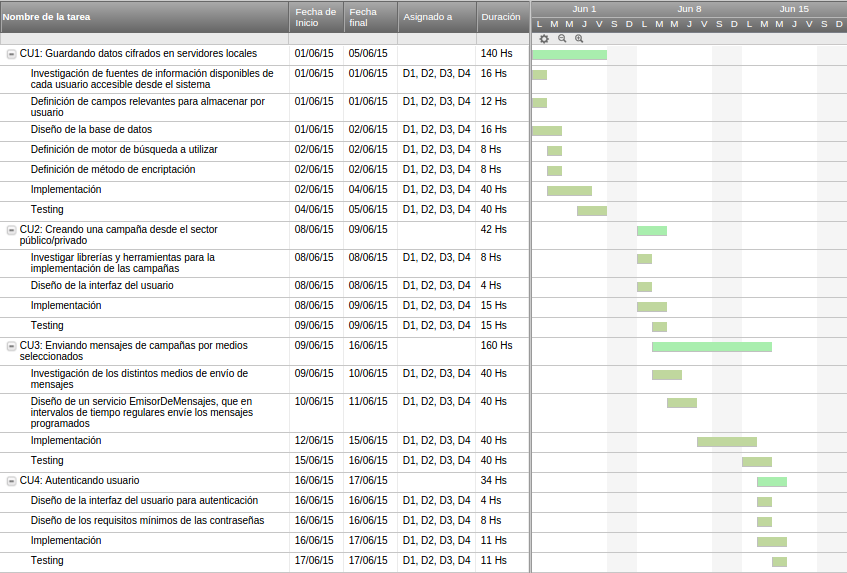
\includegraphics[width=25cm]{gantt.png}
    \caption{Diagrama de Gantt de la 1era iteración con la asignación de tiempo}
    \label{fig:gantt}
  \end{figure}
\end{center}
\end{landscape}
\newpage

%%%%%%%%%%%%%%%%%%%%%%%%%%%%%%%%%%%%%%%%%%%%%%%%%%%%%%%%%%%%%%%%%%%%%%%%%%%%%%%
%% Análisis de riesgo                                                        %%
%%%%%%%%%%%%%%%%%%%%%%%%%%%%%%%%%%%%%%%%%%%%%%%%%%%%%%%%%%%%%%%%%%%%%%%%%%%%%%%

\section{Análisis de riesgos}
\label{riesgos:r1}
\riesgo{1}
    { Los motores gráficos 2D y 3D son desarrollados por terceros. Si alguna de las dos compañías deja de funcionar, perdemos soporte para el correspondiente motor gráfico e incrementa fuertemente el costo y tiempo de desarrollo para realizar mejoras o agregar funcionalidad en el mismo. }
    {Baja} % Probabilidad
    {Alto} % Impacto
    {Media} % Exposición
    {Establecer una capa de abtracción encima de los motores gráficos para que los mismos sean reemplazables sin que sea necesario modificar los demás sistemas.} % Mitigación
    {Licitar el motor gráfico que ha perdido soporte entre nuevas empresas.} % Plan de contingencia

\riesgo{2}
    {Actualmente, los usuarios tienen múltiples modos para visualizar un partido: simulación 2D o 3D a partir del feed de la simulación, streaming de partidos reales y streaming de un render de la simulación realizado del lado del servidor. Si un usuario tiene un dispositivo sin las prestaciones necesarias para realizar una simulación de forma nativa, cada vez que tenga mala conectividad tampoco será capaz de visualizar streamings y no podrá obtener información sobre los partidos de ninguna manera. }
    {Media} % Probabilidad
    {Medio} % Impacto
    {Media} % Exposición
    {Desarrollar un feed de información acerca del partido en ejecución que sea apto para clientes con bajos recursos de hardware y mala conectividad.}
    {Proponer al usuario afectado la visualización del feed del partido basado en texto.}

\riesgo{3}
    {El sistema en su conjunto procesa varios conjuntos de datos altamente sensibles que refieren a la identidad de sus usuarios, a sus medios de pago, y la realización de las simulaciones que determinan los desafíos para bajo apuestas o con premios, así como los resultados de los mismos. Si alguno de estos sistemas es comprometido, la integridad personal o económica de los usuarios o del sistema mismo pueden sufrir consecuencias irreversibles. }
    {Media} % Probabilidad
    {Alto} % Impacto
    {Media} % Exposición
    {Investigar fuertemente las mejores prácticas en seguridad para el desarrollo de los sistemas que procesan información sensible.}
    {Suspensión inmediata de actividades en la platafoma con posibles resultados irreversibles (pagos, entrega de premios) e investigación sobre el siniestro cooperando con las autoridades.}

\newpage

\end{document}
